\documentclass[12pt]{article}
\usepackage{url,graphicx,tabularx,array,geometry,amsmath,amssymb,amsthm,bbm}
\usepackage{nips12submit_e,times}
%\usepackage[sc]{mathpazo}

\newcommand{\unionf}{\bigcup_{n=1}^{\infty} \mathcal{F}_n}
\newcommand{\F}{\mathcal{F}}
\newcommand{\E}{\mathbb{E}}
\newcommand{\PP}{\mathbb{P}}
\newcommand{\Hi}{\mathcal{H}}
\newcommand{\A}{\mathcal{A}}
\newcommand{\Aseq}{\{A_k\}_{k=1}^{\infty}}
\newcommand{\unionA}{\bigcup_{k=1}^{\infty} A_k}
\newcommand{\argmax}{\operatornamewithlimits{argmax}}

\nipsfinalcopy 

\begin{document}

\title{Unsupervised Segmentation of Multivariate Time Series Through Inertial Hidden Markov Models}

%...............................................................................
%                                   Authors
%...............................................................................
\author{
George D. Monta\~nez \\
Machine Learning Department\\
Carnegie Mellon University\\
Pittsburgh, PA USA\\
\texttt{gmontane@cs.cmu.edu} \\
\And    
Saeed Amizadeh\\
Media Sciences, Yahoo! Labs\\
Yahoo!\\
Sunnyvale, CA USA\\
\texttt{amizadeh@yahoo-inc.com} \\
\And
Nikolay Laptev \\
Media Sciences, Yahoo! Labs\\
Yahoo!\\
Sunnyvale, CA USA\\
\texttt{nlaptev@yahoo-inc.com} \\
}

\maketitle

\begin{abstract}
    Faced with the problem of segmenting a multivariate time series in an unsupervised manner, we derive two independent methods of regularizing hidden Markov models to accomplish the task. Regularization on state transitions provide smooth transitioning among states, such that the sequences are split into broad, contiguous segments. Our methods are compared to a baseline hidden Markov model, which suffers from rapid state transitioning, over-segmentation and poor performance on a segmentation task involving human activity accelerometer data from the UCI Machine Learning Repository. In comparison, the regularized methods developed here are able to perfectly segment the human activity data in 77 of 100 test cases, with accuracy of 98\% and variation of information near zero. Compared to other recent approaches, our methods provide simple, drop-in replacements for standard hidden Markov model update rules, allowing standard expectation maximization (EM) algorithms to be used for learning. Lastly, we make progress towards tuning the regularization strength in an unsupervised manner.
\end{abstract}

\section{Introduction}

This is where the introduction goes.


\section{Problem Statement}

Let $\mathbf{X} = \{\mathbf{x}_1, \ldots, \mathbf{x}_T\}$ denote a $d$-dimensional multivariate time series, where $\mathbf{x}_t \in \mathbb{R}^d$. Given such a time series, we seek to segment $\mathbf{X}$ along the time axis into \emph{segments}, where each segment corresponds to a subsequence $\mathbf{X}_{i\ldots i+m} = \{\mathbf{x}_i, \ldots, \mathbf{x}_{i+m}\}$ and maps to a predictive (latent) state $\mathbf{z}$, represented as a one-of-$K$ vector, where $|\mathbf{z}| = K$ and $\sum_{i=1}^{K}z_{t,i} = 1$. For simplicity of notation, let $\mathbf{z}_{t} = k$ denote $z_{t,k} = 1$ and let $\mathbf{Z} = \{\mathbf{z}_1, \ldots, \mathbf{z}_T\}$ denote the sequence of latent states. Then for all $\mathbf{x}_{t}$ mapping to state $k$, we require that
\begin{align*}
    \Pr(\mathbf{x}_{t+1}|\mathbf{X}_{1\ldots t}, \mathbf{z}_t = k) &= \Pr(\mathbf{x}_{t+1}| \mathbf{z}_t = k) \\
                                                                   &= \Pr(\mathbf{x}_{t'+1}| \mathbf{z}_{t'} = k) \\
                                                                   &= \Pr(\mathbf{x}_{t'+1}| \mathbf{X}_{1\ldots t'}, \mathbf{z}_{t'} = k).
\end{align*}
Thus, the conditional distribution over futures at time $t$ conditioned on being in state $k$ is equal to the distribution over futures at time $t'$ conditioned on being in the same state. Thus, we assume conditional independence given state, and stationarity of the generative process.

We impose two additional complexity criteria on our model. First, we seek models with a small number of latent states, $K \ll T$, and second, we desire state transition sequences of low complexity such that the transitioning of states does not occur too rapidly. We refer to this as the \emph{inertial transition} requirement, alluding to the physical property of matter that ensures it will continue along a fixed course unless acted upon by an external force. 

The above desiderata must be externally imposed on our model, since simply maximizing the likelihood of the data will result in $K = T$ (i.e., each sample corresponds a unique state/distribution), and in general we may have rapid transitions among states. For the first desideratum,  we choose the number of states in advance as is typically done for hidden Markov models. For the second, we directly alter the probabilistic form of our model to include a parameterized regularization that reduces the likelihood of transitioning between different latent states.

We next discuss the input and output for our problem setup.

\subsection{Problem Input}

As stated above, we are given a single $d$-dimensional multivariate time series of $T$ time samples. Alternatively, the single time series can be thought of as a collection of $d$ one-dimensional time series. As the generative story, we assume that at each time step $t$ a state $\mathbf{z}_t$ is chosen, given the previous state $\mathbf{z}_{t-1}$, according to the transition probabilities governing states. A $d$-dimensional point-sample is then drawn according to the emission density for state $\mathbf{z}_t$, and the process repeats for $1 < t \leq T$.

\subsection{Problem Output}

The output of the process is a list of integer tuples $(t, k)$, where $1 \leq t \leq T$ denotes the ending time of the segment and $1 \leq k \leq K$ the state that occurs during that segment. 

\section{Proposed Approaches}

\subsection{Baseline: $K$-state Hidden Markov Model}

As a baseline, a standard $K$-state HMM model with Gaussian emission densities is fit on the data. This model maximizes the likelihood of the data, but does not guarantee slow inertial transitioning among states. The number of states must be specified in advance, but no other parameters are needed. This gives us a starting point to improve on, allowing us to compare the regularized methods we develop.

\subsection{Maximum A Posteriori (MAP) Regularized HMM}

Following~\cite{MAP1994}, we alter the standard HMM to include a Dirichlet prior on the transition probability matrix, such that transitions out-of-state are penalized by some regularization factor. A Dirichlet prior on the transition matrix $\mathbf{A}$, for the $j$th row, has the form
\begin{align*}
    p(A_j; \eta) &\propto \prod_{i=1}^{K} A_{jk}^{\eta_{jk}}
\end{align*}
where the $\eta_{jk}$ are free parameters and $A_{jk}$ is the transition probability from state $j$ to state $k$. The posterior joint density over $\mathbf{X}$ and $\mathbf{Z}$ becomes
\begin{align*}
    P(\mathbf{X}, \mathbf{Z} ; \mathbf{\theta}, \eta) 
    &\propto \left[\prod_{i=1}^{K}\prod_{i=1}^{K} A_{jk}^{\eta_{jk} - 1}\right] P(\mathbf{X}, \mathbf{Z} \mid \mathbf{A}; \mathbf{\theta}) 
\end{align*}
and the log-likelihood is
\begin{align*}
\ell(\mathbf{X}, \mathbf{Z} ; \mathbf{\theta}, \eta) 
&\propto \sum_{i=1}^{K}\sum_{i=1}^{K} (\eta_{jk} - 1)\log A_{jk} + \log P(\mathbf{z}_{1}; \theta) + \sum_{t=1}^{T}\log P(\mathbf{x}_t|\mathbf{z}_t; \mathbf{\theta}) + \sum_{t=2}^{T}\log P(\mathbf{z}_t|\mathbf{z}_{t-1}; \mathbf{\theta}).
\end{align*}

We then use MAP estimation in the M-step of the EM algorithm, to update the transition probability matrix. Maximizing, we obtain the update equation for the transition matrix, namely
\begin{align*}
    A_{jk} &= \frac{(\eta_{jk} - 1) + \sum_{t=2}^{T} \xi(z_{(t-1)j}, z_{tk})}   
    {\sum_{i=1}^{K}(\eta_{ji} - 1) + \sum_{i=1}^{K}\sum_{t=2}^{T} \xi(z_{(t-1)j}, z_{ti})}.
\end{align*}

Although we have a tractable, efficient algorithm for learning the regularized HMM and, given our prior, we can control the probability of self-transitions among states, this method requires that we choose a set of $K^2$ parameters for the Dirichlet prior. However, since we are solely concerned about increasing the probability of self-transitions, we can reduce these parameters to a single parameter $\lambda$ governing the amplification of self-transitions. We therefore define $\eta_{jk} = 1$ when $j\not=k$ and $\eta_{kk}= \lambda \geq 1$ otherwise, and the transition update equation becomes
\begin{align*}
    A_{jk} &= \frac{(\lambda - 1)^{\mathbbm{1}(j = k)} + \sum_{t=2}^{T} \xi(z_{(t-1)j}, z_{tk})}   
    {(\lambda - 1) + \sum_{i=1}^{K}\sum_{t=2}^{T} \xi(z_{(t-1)j}, z_{ti})}
\end{align*}
where $\mathbbm{1}(\cdot)$ denotes the indicator function.

\subsubsection{Scale-Free MAP Regularization}

Astute readers may notice that the strength of the regularization diminishes with growing $T$, so that asymptotically the regularized estimates and unregularized estimates become equivalent. Figure~\ref{fig:short-real-data} shows a regularized segmentation of human accelerometer data (discussed later in the Experiments section), where the regularization is strong enough to correctly segment the series into large, contiguous sections. If we then increase the number of data points in each section by a factor of ten while keeping the same regularization parameter setting, we see that the regularization is no longer strong enough, as is shown in Figure~\ref{fig:long-real-data}. Two of the sections have become splintered into small, choppy regions. Thus, the $\lambda$ parameter is sensitive to the size of the time series.

\begin{figure}[htbp]
  \caption{Human activities accelerometer data, short sequence. Vertical partitions correspond to changes of state. Only one dimension of data is shown.}
  \centering
    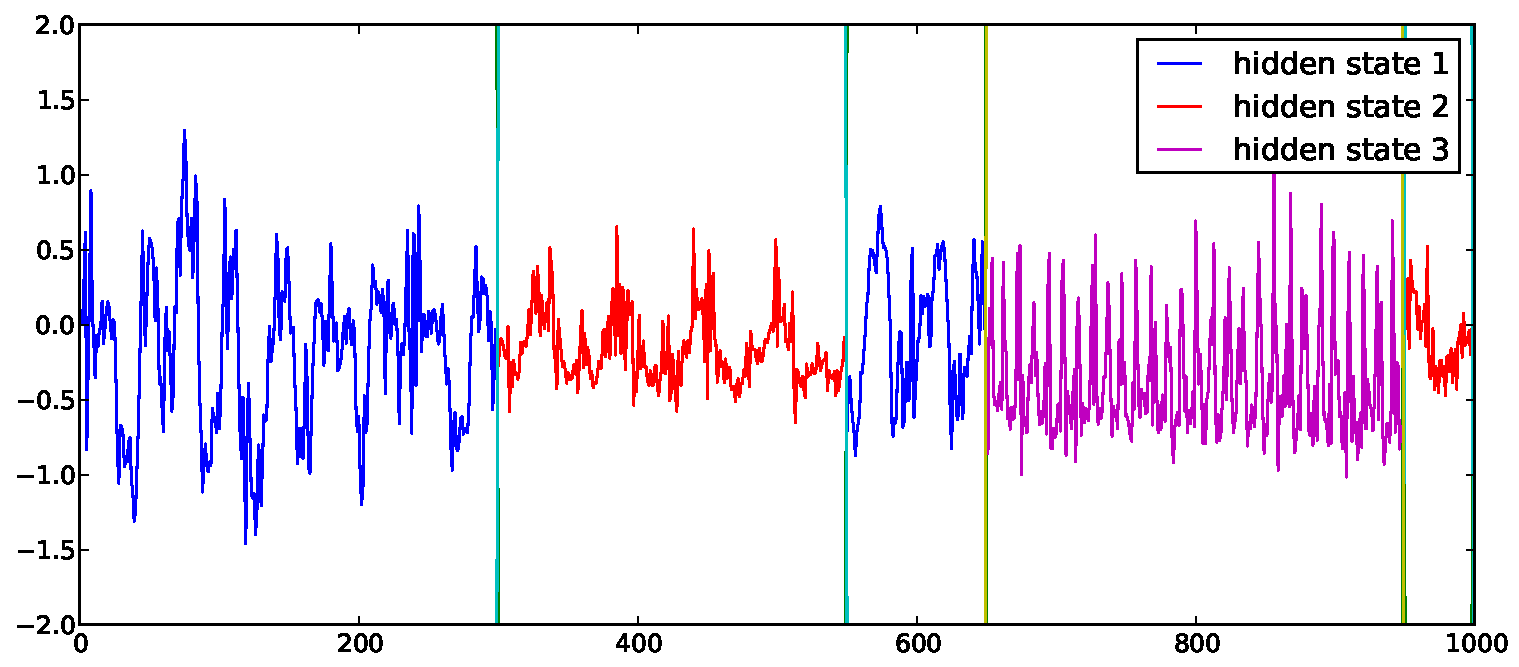
\includegraphics[width=0.8\linewidth]{images/MAP_results_hard_activity_short_3_states.pdf}
    \label{fig:short-real-data}
\end{figure}

\begin{figure}[htbp]
  \caption{Human activities accelerometer data, long sequence. Regularization parameter from short sequence used here.}
  \centering
    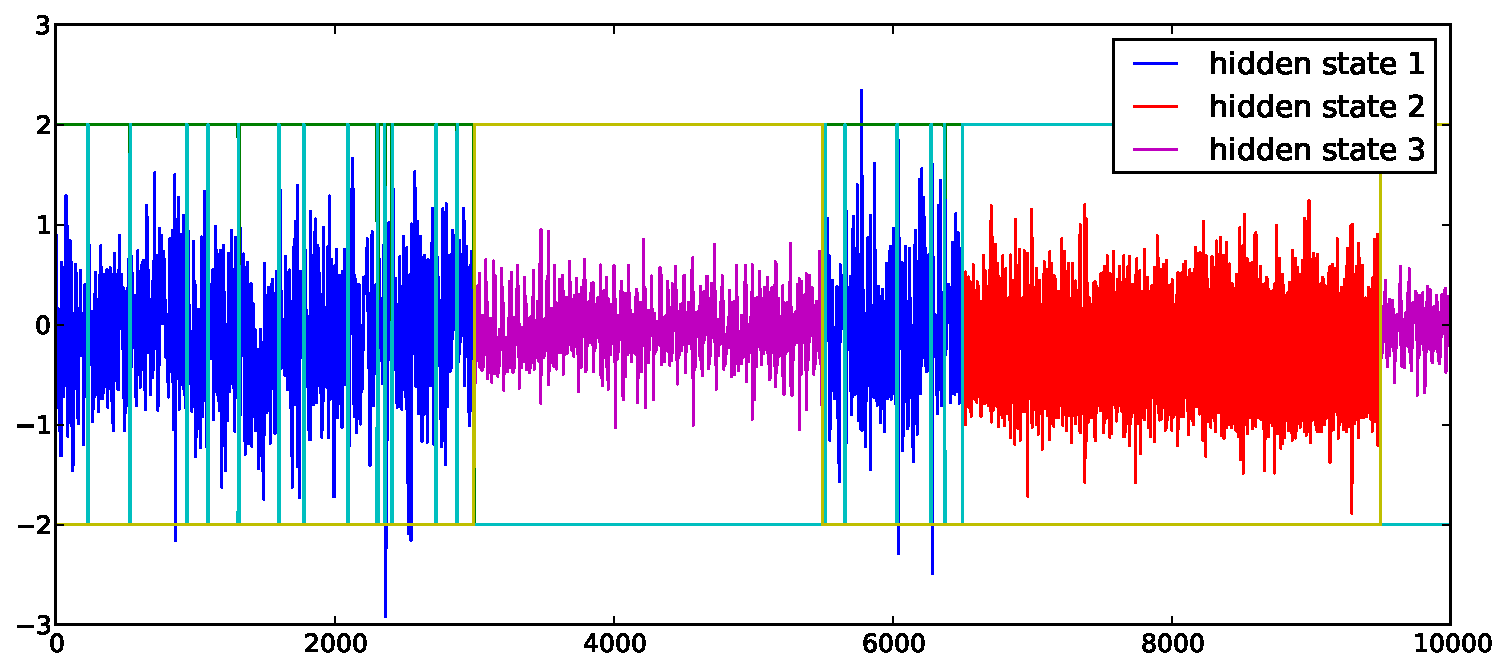
\includegraphics[width=0.8\linewidth]{images/MAP_results_hard_activity_long_3_states.pdf}
    \label{fig:long-real-data}
\end{figure}

We desire a model where the regularization strength is scale-free, having roughly the same strength regardless of how the time series grows. To achieve this, we define the $\lambda$ parameter to scale with the number of transitions, namely $\lambda = (T-1)^\zeta$, and our scale-free update equation becomes
\begin{align*}
    A_{jk} &= \frac{((T - 1)^{\zeta}-1)^{\mathbbm{1}(j = k)} + \sum_{t=2}^{T} \xi(z_{(t-1)j}, z_{tk})}   
    {((T - 1)^{\zeta} - 1) + \sum_{i=1}^{K}\sum_{t=2}^{T} \xi(z_{(t-1)j}, z_{ti})}.
\end{align*}
This preserves the effect of regularization as $T$ increases, and $\zeta$ becomes our new regularization parameter, controlling the strength of the regularization. Figures~\ref{fig:short-real-data-scale-free} and \ref{fig:long-real-data-scale-free} shows the scale-free regularized result on both a short and long sequence, using the same regularization parameter. The parameter was chosen in reference to the short sequence, selecting the smallest parameter that still provided correct segmentation. As can be seen, the regularization strength is sufficient for the long sequence as well, illustrating the effectiveness of a scale-free parameterization.

\begin{figure}[htbp]
  \caption{Human activities accelerometer data, short sequence, with minimum scale-free regularization parameter.}
  \centering
    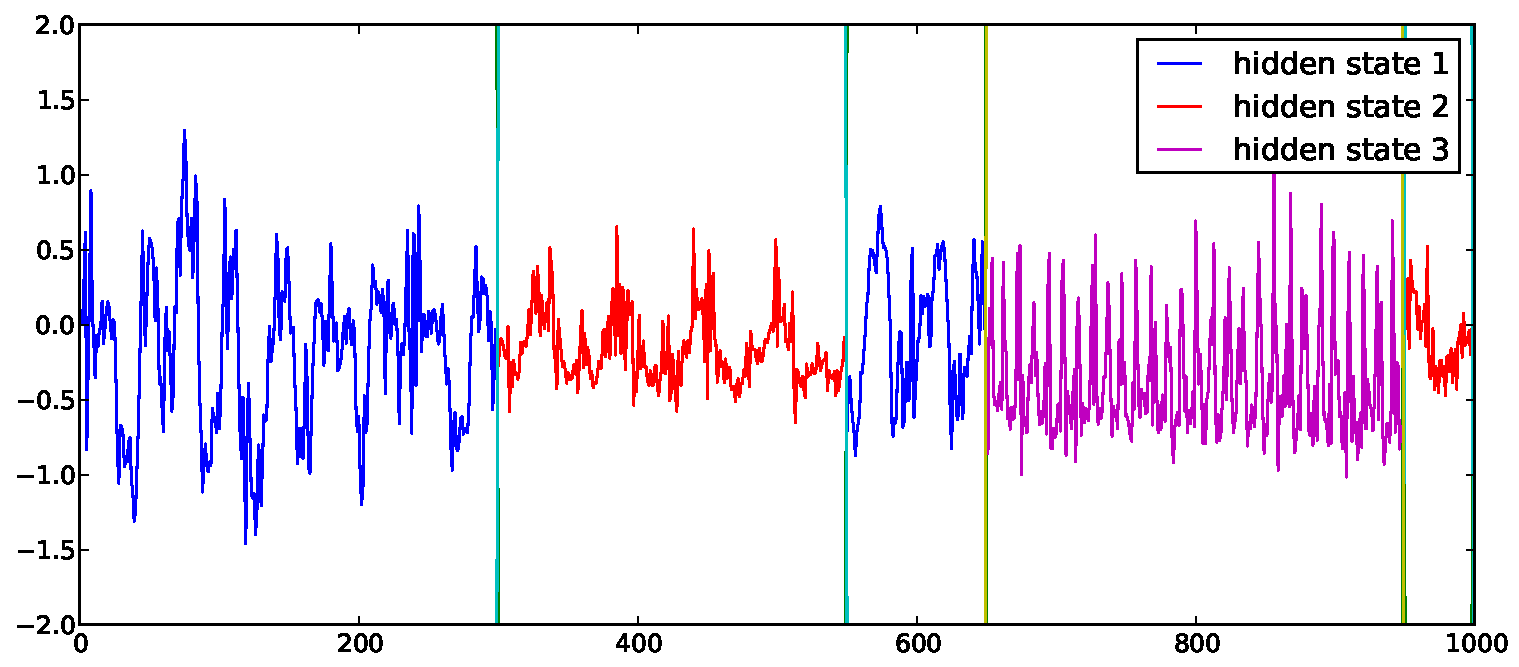
\includegraphics[width=.8\linewidth]{images/MAP_SCALE_FREE_results_hard_activity_short_3_states.pdf}
    \label{fig:short-real-data-scale-free}
\end{figure}

\begin{figure}[htbp]
  \caption{Human activities accelerometer data, long sequence, with minimum scale-free regularization parameter chosen in regards to short sequence. Correct segmentation is maintained despite the length of the time series increasing by an order of magnitude.}
  \centering
    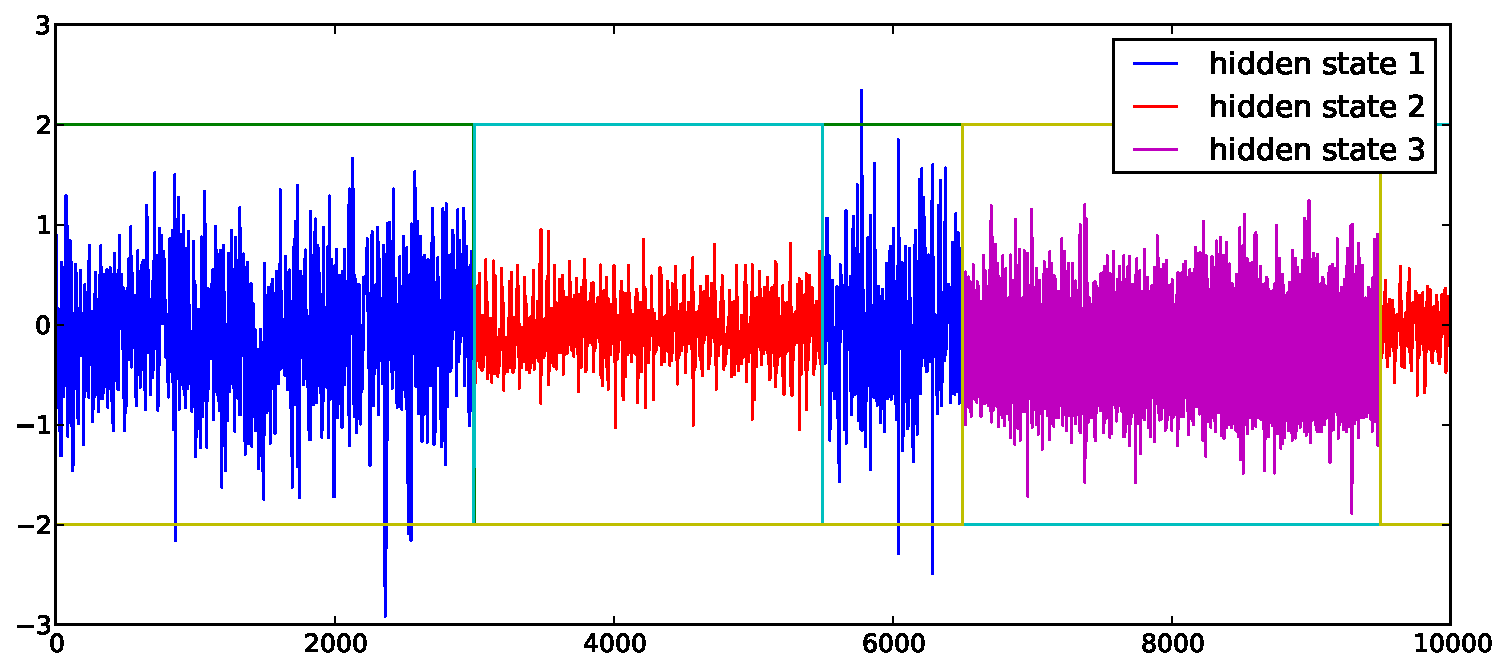
\includegraphics[width=.8\linewidth]{images/MAP_SCALE_FREE_results_hard_activity_long_3_states.pdf}
    \label{fig:long-real-data-scale-free}
\end{figure}

\subsubsection{Inertial Regularization via Pseudo-observations}

We now derive a second method of regularizing the state transitions, where we alter the HMM likelihood function to include a fictional observation, $V$. This is a binary random variable indicating that a transition was chosen at random from among all transitions, according to some distribution, and that the transition observed was a self-transition. Thus, we view the transitions as being partitioned into two sets, self-transitions and non-self-transitions, and we draw a member of the self-transition set according to a Bernoulli distribution governed by some parameter $p$. Given a latent state sequence $\mathbf{Z}$, with transitions chosen according to transition matrix $\mathbf{A}$, we define $p$ as a function of both $\mathbf{Z}$ and $\mathbf{A}$. We would like $p$ to have two properties: 1) it should increase with increasing $\sum_k A_{kk}$ (probability of self-transitions) and 2) it should increase as the number of self-transitions in $\mathbf{Z}$ increases. This will allow us to encourage self-transitions as a simple consequence of maximizing the likelihood of our observations.

We begin with a version of $p$ based on a penalization constant $0 < \epsilon < 1$ that scales appropriately with the number of self-transitions. If we raise $\epsilon$ to a large positive power, the resulting $p$ will decrease. Thus, we define $p$ as $\epsilon$ raised to the number of non-self-transitions in the state transition sequence, so that the probability of selecting a self-transition increases as the number of non-self-transitions decreases. Using the fact that the number of non-self-transitions equals $(T-1) - \sum^{T}_{t=2}\sum^{K}_{k=1}z_{(t-1)k}z_{tk}$, we obtain 
\begin{align}
    p &= \epsilon^\text{\tiny NUM.\ OF NON-SELF-TRANSITIONS}\\
      &= \epsilon^{(T-1) - \sum^{T}_{t=2}\sum^{K}_{k=1}z_{(t-1)k}z_{tk}} \notag\\
      &= \epsilon^{\sum^{T}_{t=2}1 - \sum^{T}_{t=2}\sum^{K}_{k=1}z_{(t-1)k}z_{tk}} \notag\\
      &= \epsilon^{\sum^{T}_{t=2}\sum^{K}_{k=1}z_{(t-1)k} - \sum^{T}_{t=2}\sum^{K}_{k=1}z_{(t-1)k}z_{tk}} \notag\\
      &= \epsilon^{\sum^{T}_{t=2}\sum^{K}_{k=1}z_{(t-1)k} - z_{(t-1)k}z_{tk}} \notag\\
      &= \prod^{T}_{t=2}\prod_{k=1}^{K}\epsilon^{z_{(t-1)k} - z_{(t-1)k}z_{tk}}. \label{eq:eps-0}
\end{align}

Since $\epsilon$ is arbitrary, we choose $\epsilon = A_{kk}$, to allow $p$ to scale appropriately with increasing probability of self-transition. We therefore arrive at
\begin{align*}
    p &= \prod^{T}_{t=2}\prod^{K}_{k=1}A_{kk}^{z_{(t-1)k} - z_{(t-1)k}z_{tk}}.
\end{align*}
Thus, we define $p$ as a computable function of $\mathbf{Z}$ and $\mathbf{A}$. Defining $p$ in this deterministic manner is equivalent to choosing the parameter value from a degenerate probability distribution that places a single point mass at the value computed, allowing us to easily obtain a posterior distribution on $V$. Furthermore, we see that the function increases as the number of self-transitions increases, since $A_{kk} \leq 1$ for all $k$, and $p$ will generally increase as $\sum_k A_{kk}$ increases. Thus, we obtain a parameter $p \in (0,1]$ that satisfies all our desiderata.

With $p$ in hand, we say that $V$ is drawn according to the Bernoulli distribution, Bern($p$), and we observe $V = 1$ (i.e., a member of the self-transition set was chosen). Since $P(V = 1|\mathbf{Z};\mathbf{A}) = p$, we have
\begin{align*}
    P(V = 1|\mathbf{Z}; \mathbf{A}) &= \prod^{T}_{t=2}\prod^{K}_{k=1}A_{kk}^{z_{(t-1)k} - z_{(t-1)k}z_{tk}}.
\end{align*}
To gain greater control over the strength of regularization, let $\lambda$ be a positive integer and $\mathbf{V}$ be an $\lambda$-length sequence of pseudo-observations, drawn i.i.d.\ according to Bern($p$). Thus, 
\begin{align*}
    P(\mathbf{V} = \mathbf{1}|\mathbf{Z}; \mathbf{A}) &= \left[\prod^{T}_{t=2}\prod^{K}_{k=1}A_{kk}^{z_{(t-1)k} - z_{(t-1)k}z_{tk}}\right]^\lambda
\end{align*}
where $\mathbf{1}$ denotes the all-ones sequence of length $\lambda$.

Clearly $\mathbf{V}$ is conditionally independent of $\mathbf{X}$ given the latent state sequence $\mathbf{Z}$. We now consider the joint density over $\mathbf{X}$, $\mathbf{V}$, and $\mathbf{Z}$, making use of our conditional independence assumption. We parameterize the joint density by $\mathbf{\theta} = \{\mathbf{\pi},\mathbf{A}, \mathbf{\phi}\}$, which are the start-state probabilities, state transition matrix and emission parameters, respectively. We have
\begin{align*}
    P(\mathbf{X}, \mathbf{V}, \mathbf{Z} ; \mathbf{\theta}) 
    &= P(\mathbf{V}|\mathbf{Z}; \mathbf{\theta}) P(\mathbf{z}_{1} ; \theta) \left[\prod_{t=1}^{T}P(\mathbf{x}_t|\mathbf{z}_t; \mathbf{\theta})\right]\left[\prod_{t=2}^{T}P(\mathbf{z}_t|\mathbf{z}_{t-1}; \mathbf{\theta})\right]
\end{align*}
and, taking the log of the likelihood,
\begin{align*}
    \ell(\mathbf{X}, \mathbf{V}, \mathbf{Z} ; \mathbf{\theta}) 
    &= \log P(\mathbf{V}|\mathbf{Z}; \mathbf{\theta}) + \log P(\mathbf{z}_{1}; \theta) + \sum_{t=1}^{T}\log P(\mathbf{x}_t|\mathbf{z}_t; \mathbf{\theta}) + \sum_{t=2}^{T}\log P(\mathbf{z}_t|\mathbf{z}_{t-1};\mathbf{\theta}).
\end{align*}

Noting that 
\begin{align*}
    P(\mathbf{z}_{1}; \theta) &= \prod_{k=1}^{K}\pi_{k}^{z_{1k}}, \\
    P(\mathbf{x}_t|\mathbf{z}_t; \mathbf{\theta}) &= \prod_{k=1}^{K} P(\mathbf{x}_t ; \mathbf{\phi}_k)^{z_{tk}},\text{ and }\\ 
    P(\mathbf{z}_t|\mathbf{z}_{t-1}; \mathbf{\theta}) &= \prod_{k=1}^{K}\prod_{j=1}^{K}A_{jk}^{z_{(t-1)j}z_{tk}},
\end{align*}
and substituting into $\ell(\mathbf{X}, \mathbf{V}, \mathbf{Z} ; \mathbf{\theta})$ we obtain
\begin{align*}
    \ell(\mathbf{X}, \mathbf{V}=\mathbf{1}, \mathbf{Z} ; \mathbf{\theta}) 
    &= \sum^{T}_{t=2}\sum^{K}_{k=1}\lambda[z_{(t-1)k} - z_{(t-1)k}z_{tk}]\log A_{kk} + \sum_{k=1}^{K}{z_{1k}}\log \pi_{k} \notag\\
    &+ \sum_{t=1}^{T}\sum_{k=1}^{K} z_{tk}\log P(\mathbf{x}_t ; \mathbf{\phi}_k) + \sum_{t=2}^{T}\sum_{k=1}^{K}\sum_{j=1}^{K}[z_{(t-1)j}z_{tk}]\log A_{jk}.
\end{align*}

Following Bishop~\cite{bishop2007pattern}, we define
\begin{align*}
    \gamma(z_{tk}) &= \mathbb{E}[z_{tk}] = \sum_{\mathbf{z}}\gamma(\mathbf{z})z_{tk} \\
    \xi(z_{(t-1)j}, z_{tk}) &= \mathbb{E}[z_{(t-1)j}z_{tk}] = \sum_{\mathbf{z}}\gamma(\mathbf{z})z_{(t-1)j}z_{tk}
\end{align*}
to obtain
\begin{align}\label{eq:main}
    \mathbb{E}_{\mathbf{Z}}[\ell(\mathbf{X}, \mathbf{V}=\mathbf{1}, \mathbf{Z} ; \mathbf{\theta})]
    &= \sum^{T}_{t=2}\sum^{K}_{k=1}\lambda[\gamma(z_{(t-1)k})-\xi(z_{(t-1)k}, z_{tk})]\log A_{kk} + \sum_{k=1}^{K}\gamma(z_{1k})\log \pi_{k} \notag\\
    &+ \sum_{t=1}^{T}\sum_{k=1}^{K} \gamma(z_{tk})\log P(\mathbf{x}_t ; \mathbf{\phi}_k) + \sum_{t=2}^{T}\sum_{k=1}^{K}\sum_{j=1}^{K}\xi(z_{(t-1)j}, z_{tk})\log A_{jk}.
\end{align}

Using Lagrange multipliers, taking the derivative of (\ref{eq:main}) with respect to $A_{jk}$ and setting to the result to zero, we obtain the regularized maximum likelihood estimate for $A_{jk}$, namely
\begin{align*}
    A_{jk} &= \frac{\sum_{t=2}^{T} \xi(z_{(t-1)k}, z_{tk}) + \sum_{t=2}^{T}{\mathbbm{1}(j = k)}\lambda[\gamma(z_{(t-1)k}) - \xi(z_{(t-1)k}, z_{tk})]}   
    { \sum_{t=2}^{T} \sum_{i=1}^{K} \left(\xi(z_{(t-1)j}, z_{ti}) + {\mathbbm{1}(j = i)}\lambda[\gamma(z_{(t-1)i}) - \xi(z_{(t-1)i}, z_{ti})]\right)}
\end{align*}
where $\mathbbm{1}(\cdot)$ denotes the indicator function. The forward-backward algorithm can then be used for efficient computation of the $\gamma$ and $\xi$ values, as is the case for unregularized HMMs.

Ignoring normalization, we see that
\begin{align*}
    A_{jk} &\propto \begin{cases} 
                \sum_{t=2}^{T} \xi(z_{(t-1)k}, z_{tk}) + \lambda\sum_{t=2}^{T}[\gamma(z_{(t-1)k}) - \xi(z_{(t-1)k}, z_{tk})] & \mbox{if } j=k \\ 
                \sum_{t=2}^{T} \xi(z_{(t-1)j}, z_{tk}) & \mbox{otherwise.}
              \end{cases}
\end{align*}
Thus, $\lambda$ is a multiplier of additional mass contributions for self-transitions, where the contributions are the difference between $\gamma(z_{(t-1)k})$ and $\xi(z_{(t-1)k}, z_{tk})$. These two quantities represent, respectively, the expectation of being in a state $k$ at time $t-1$ and the expectation of remaining there in the next time step. The larger $\lambda$ or the larger the difference between arriving at a state and remaining there, the greater the additional mass given to self-transition. 

Similar to the MAP case, we let $\lambda = (T-1)^{\zeta}$ to maintain consistent regularization strength in the face of increasing sequence length, where $\zeta$ becomes our new regularization parameter.


\subsubsection{Towards Parameter-Free Regularization}\label{sec:param-free}

Our methods of inertial transition regularization work well as long as the strength of regularization is provided. Here we seek to develop a version of the regularized HMM that does not require specification in advance of the regularization parameter. We accomplish this by making an assumption concerning the distribution of segment lengths. If we assume that most of the segment lengths are of roughly the same order-of-magnitude scale, then for a fixed $K$, we can automatically tune the regularization parameter.

We first define a range of possible regularization parameter values (such as $\lambda \in [0, 5]$), and perform a search on this interval for a value that gives sufficient regularization. ``Sufficient regularization'' is defined with regards to the Gini ratio~\cite{gini1936,wiki:1}, which is a measure of statistical dispersion often used to quantify income inequality. For a collection of observed segment lengths $L = \{l_1, \ldots, l_m\}$, given in ascending order, the Gini ratio is estimated by
\begin{align*}
    G(L) &= 1 - \frac{2}{m-1}\left(m - \frac{\sum_{i=1}^{m} i l_i}{\sum_{i=1}^{m} l_i}\right)
\end{align*}


Our assumption is that the true segmentation has a Gini ratio less than one-half, which corresponds to having more equality among segment lengths than not. 

We perform a binary search on our search interval, and for each parameter we train a model and evaluate the Gini ratio of the computed segment lengths. If the ratio is greater than one-half, we restrict ourselves to the upper interval and recurse. If the ratio is less than one-half, we store the current parameter value, reduce the parameter space to the lower interval and recurse. At the base of our recursion, we see if the interval width is smaller than some $\epsilon$ value, then return the parameter. On returning, we pass back the result from the recursion branch we took. As a special case, when the current parameter value has satisfied the Gini ratio condition but the left-branch recursion has not, we return the current parameter value rather than the child recursion value. Doing this guarantees that the algorithm will return the smallest regularization parameter value satisfying the Gini coefficient criterion, if such a value exists in the search space. Thus we have a parameter-free method of regularizing the segmentation task, at a cost of increasing runtime complexity by a factor of $O(\log_2 (R / \epsilon))$, where $R$ is the range of the parameter space.

\section{Experiments}\label{sec:Experiments}

We perform two segmentation tasks on simulated and real multivariate time series data, using our scale- and parameter-free regularized HMM. For comparison, we present the results of applying a standard $K$-state hidden Markov model, where the correct number of states $K$ is provided for both models. We also test the result from providing an incorrect number of states to both models, where we can see the positive effects of including regularization even when the correct number of states is not known. Per the models used, we performed all tasks in an unsupervised manner, with state labels being used only for evaluation.

\subsection{Data}\label{sec:datasets}

Our simulated dataset consists of twenty-thousand time points of twenty dimensional data (20D), generated using two latent state multivariate Gaussians with unit covariance and differing means. State 1 is mean zero, whereas State 2 has unit mean. The data are generated from the first Gaussian for 3,333 time points, then from the second for the next 3,333 points, then the final 3,334 are generated again from the first Gaussian. This provides a simple test case for the two methods. Figure~\ref{fig:simulated} shows the simulated data and states that generated them.

\begin{figure}[htbp]
  \caption{Simulated two-state, 20-dimensional multivariate data.}
  \centering
    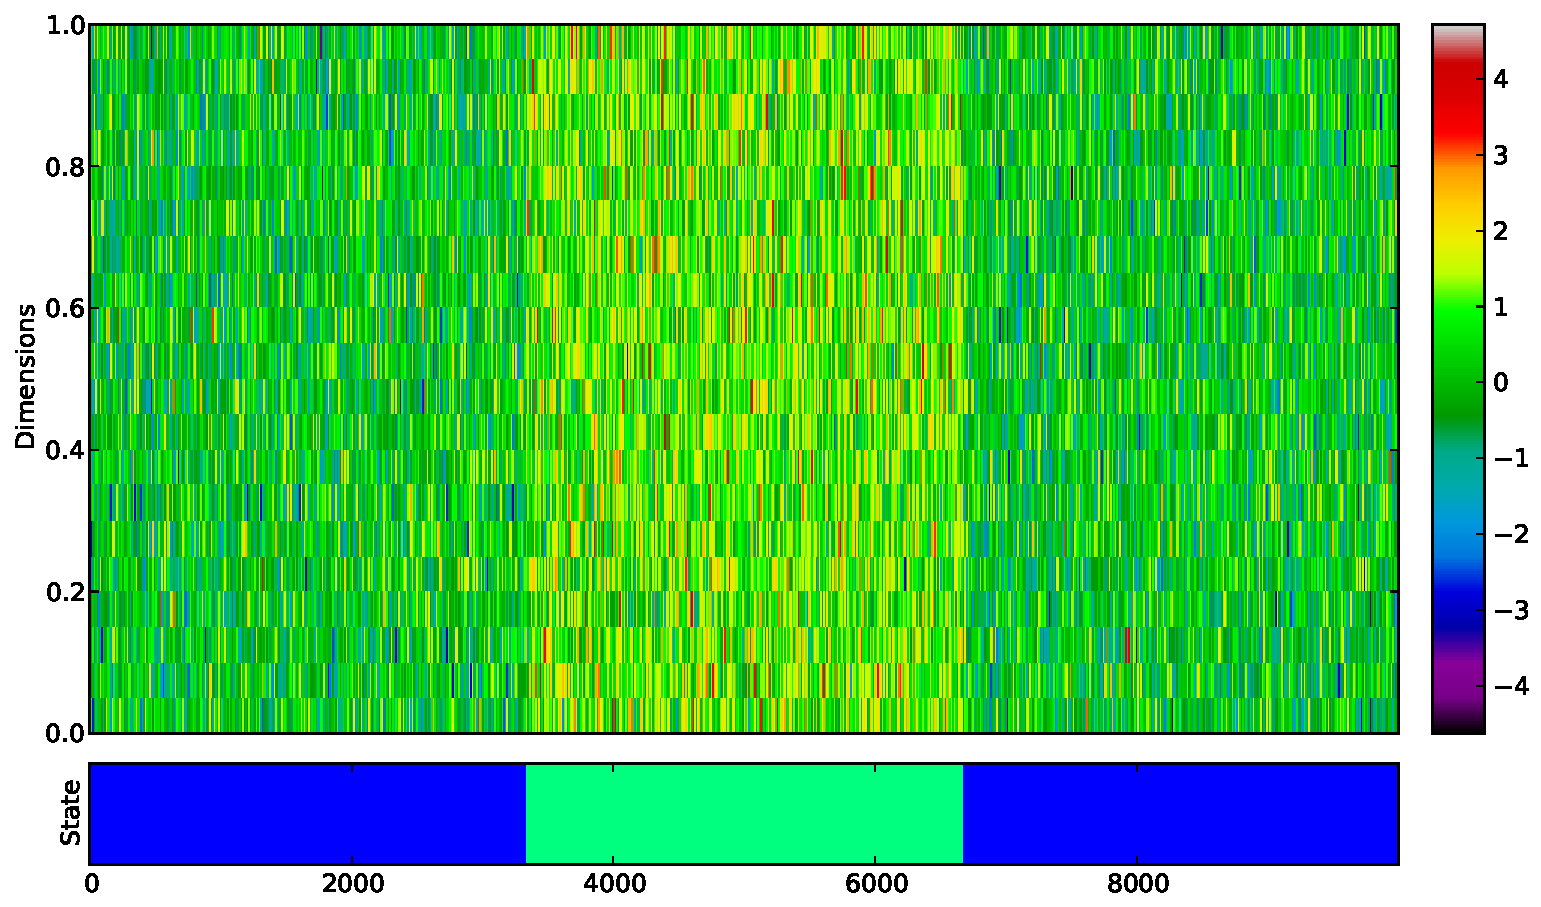
\includegraphics[width=1.\linewidth]{images/2-state-simulated-data.pdf}
    \label{fig:simulated}
\end{figure}

\begin{figure}[htbp]
  \caption{Human activities accelerometer data. Three state, 45-dimensional.}
  \centering
    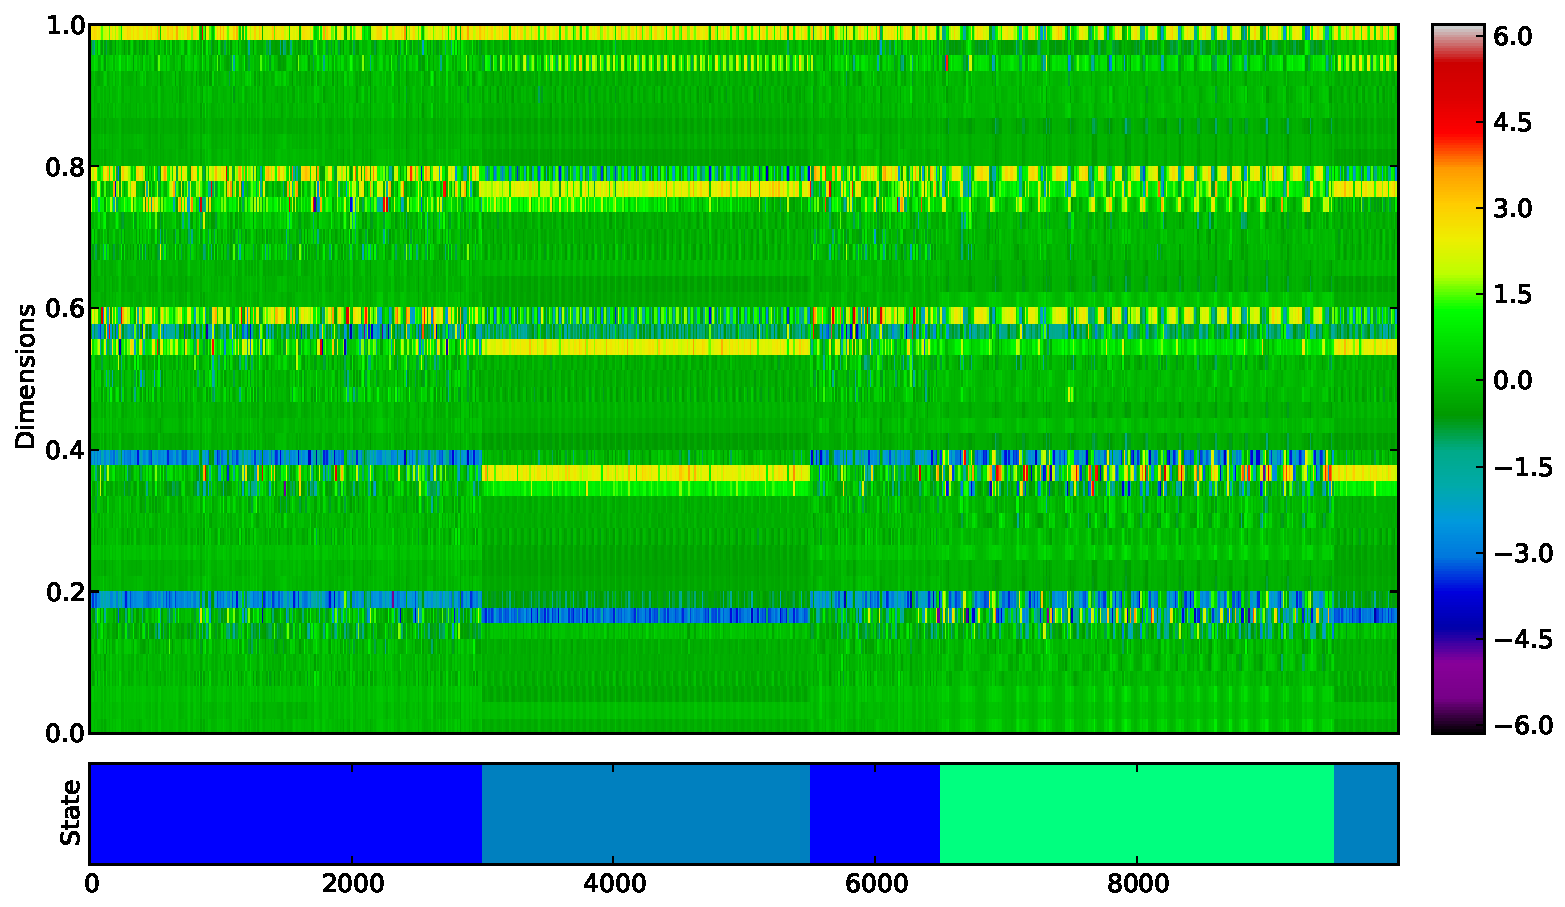
\includegraphics[width=1.\linewidth]{images/accelerometer-data.pdf}
    \label{fig:accelerometer}
\end{figure}

The second dataset is generated from real-world forty-five dimensional (45D) human accelerometer data~\cite{Altun:2010:CSC:1823245.1823314} recorded for users performing five different activities, namely, playing basketball, rowing, jumping, ascending stairs and walking in a parking lot. We generated one hundred multivariate times series from the underlying dataset, with varying activities (latent states) and number of segments. To generate these sets, we chose among the five different activities and chose anywhere from two to twenty segments. The process was as follows. First, we chose the number of segments, uniformly from $\{2, \ldots, 20\}$. Then, for each segment, we chose an activity uniformly at random from among the five possible, and selected a segment length proportion of between 5\% and 50\%. The selected number of corresponding time points were extracted from the activity (keeping track of position in the sequence, and modulo the length of the sequence), rescaled to zero mean and unit variance, and appended to the output sequence. The final output sequence was truncated to ten thousand time points, or discarded if the sequence contained fewer than ten thousand points or fewer than two distinct activities. This resulted in a multivariate time series of fixed length, with varying number of segments, activities and segment lengths. The process was repeated to generate one hundred such time series of ten thousand time points each used in the quantitative analysis described in Section~\ref{sec:quantitative}. An example of such generated data sequences is shown in Figure~\ref{fig:accelerometer}.

\subsection{Methodology}

We compared performance of a standard $K$-state hidden Markov model with our regularized MAP HMM on the two datasets described in the previous section. For the second dataset, we performed a quantitative analysis, treating the task as a multi-class classification problem, and measured the minimum zero-one loss under all possible permutations of output labels, to accommodate the fact that the output labels of an HMM may be a permuted mapping of the true labels. We measured the normalized variation of information~\cite{meila} between the predicted state sequence and true state sequence, which is an information metric capturing the symmetric two-way conditional entropy between two partitionings (clusterings) of a sequence.  In addition to this, we considered the ratio of predicted number of segments to true number of segments, which gives us a sense of whether a method over- or under-segments data, and the absolute segment number ratio (ASNR), which is defined as
\[
    \text{ASNR} = \frac{\max(S_t, S_p)}{\min(S_t, S_p)}
\]
where $S_t$ is the true number of segments in the sequence and $S_p$ is the predicted number of segments. This value tells us how much a segmentation method diverges from the ground truth in terms of relative factor of segments. Lastly, we tracked the number of segments difference between the predicted segmentation and true segmentation and how many segmentations we done perfectly, giving the correct states at all correct positions.

To speed up evaluation, we used a fixed MAP regularization parameter for each set of tests ($\zeta = 73$), which is the largest regularization value capable of being used on the test system. As the parameter value decreases, we get performance more similar to the standard HMM, where performance is identical for $\zeta = 0$ and $\zeta = 1$, for MAP and pseudo-observation regularization, respectively.

\section{Results}

\subsection{Simulated Data Results}

Both methods perform well on the simulated dataset. The standard HMM correctly segments the data into the latent state segments, without the need for regularization. Thus, we should expect our parameter-free regularization method to also correctly segment the series and select a small regularization parameter value.

Figure~\ref{fig:sim-results-MAP} shows the result of the regularized HMM, which also correctly segments the series. Time series data from a single dimension is displayed, for ease of visualization. The final parameter value found was $\zeta = 0.005$, using an epsilon of 0.01. (Thus the final $\zeta$ is simply the smallest regularization value permissible, being the center of the interval $[0,0.01]$.) Thus, our method performs as expected on the simple simulated test case and discovers the correct regularization parameter.

\begin{figure}[htbp]
  \caption{Segmentation of two-state simulated data using regularized MAP HMM.}
  \centering
    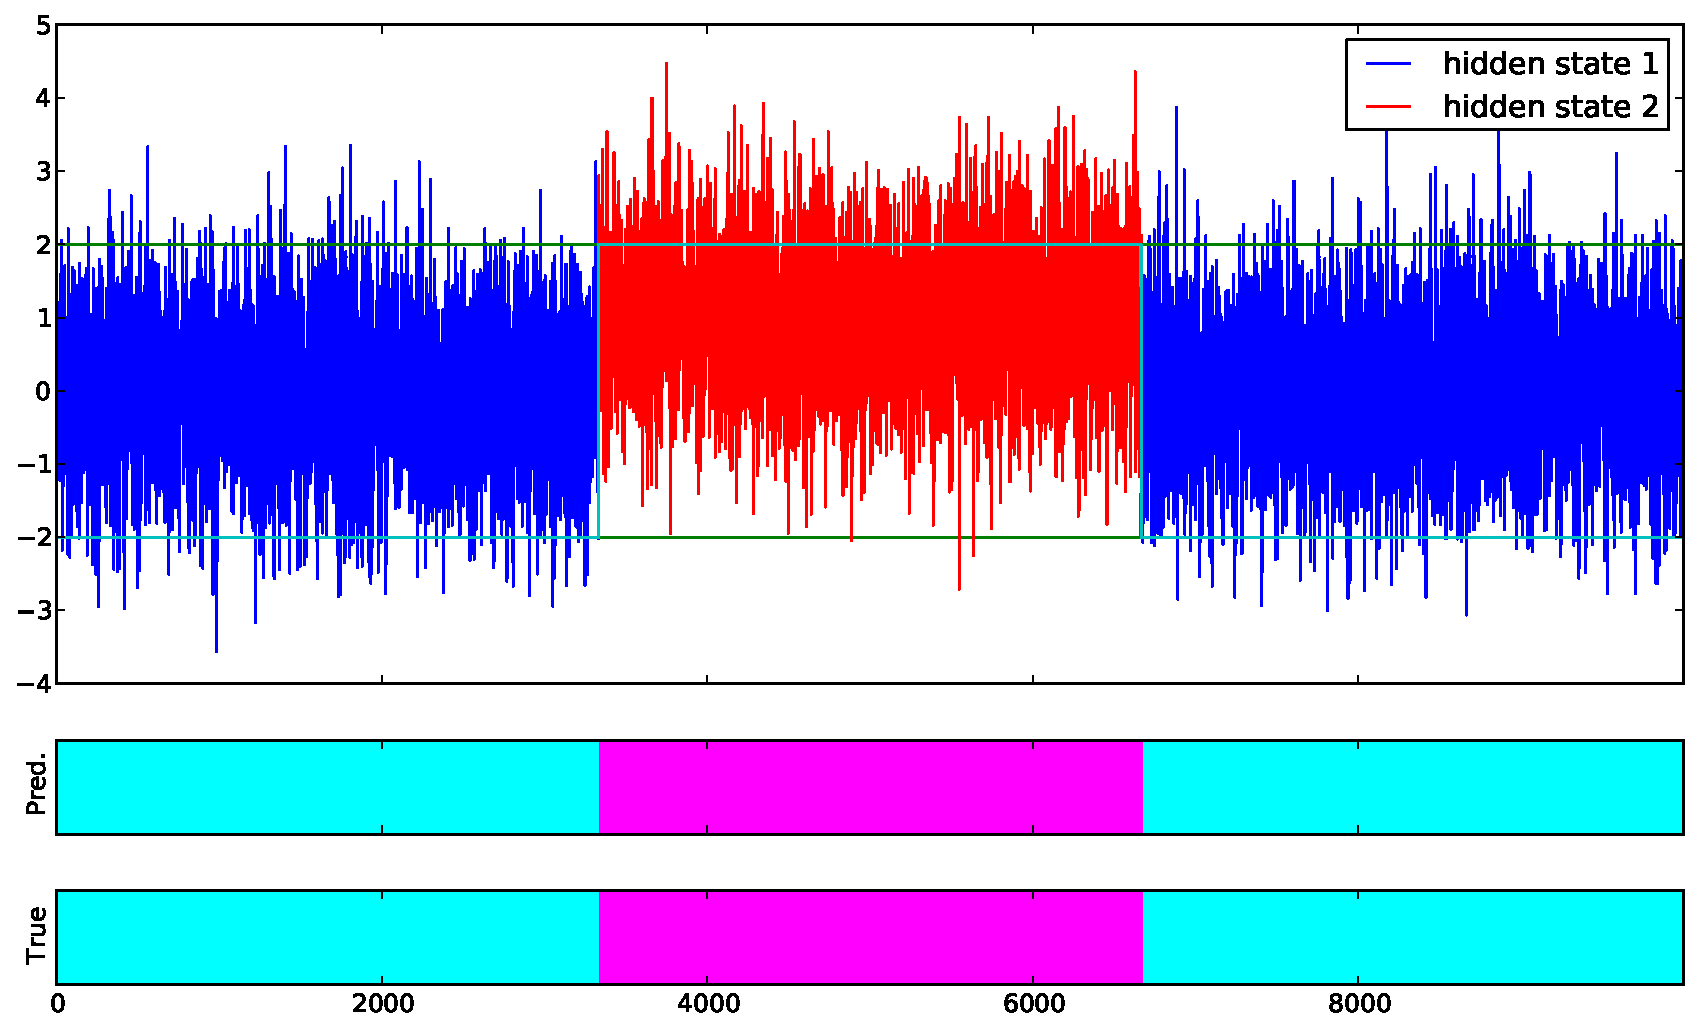
\includegraphics[width=.8\linewidth]{images/MAP_PARAM_FREE_results_sim_data_0,00_2_states.pdf}
    \label{fig:sim-results-MAP}
\end{figure}

\subsection{Human Activities Accelerometer Data Results}\label{sec:quantitative}

As an example of performance on the forty-five dimensional human activities accelerometer data, Figure~\ref{fig:real-results-MAP} shows the segmentation results for the MAP regularized HMM on a typical sequence, displaying a single dimension of the multivariate time series for clarity. The regularized MAP HMM correctly segments the time series, as can be seen from the congruence between the true and predicted state transition histories (bottom of Figure~\ref{fig:real-results-MAP}). A final parameter value of $\zeta = 1.97$ was automatically discovered through the search process described in Section~\ref{sec:param-free}, and results are shown for that parameter value.

\begin{figure}[htbp]
  \caption{Segmentation of human activities accelerometer data using regularized MAP HMM.}
  \centering
    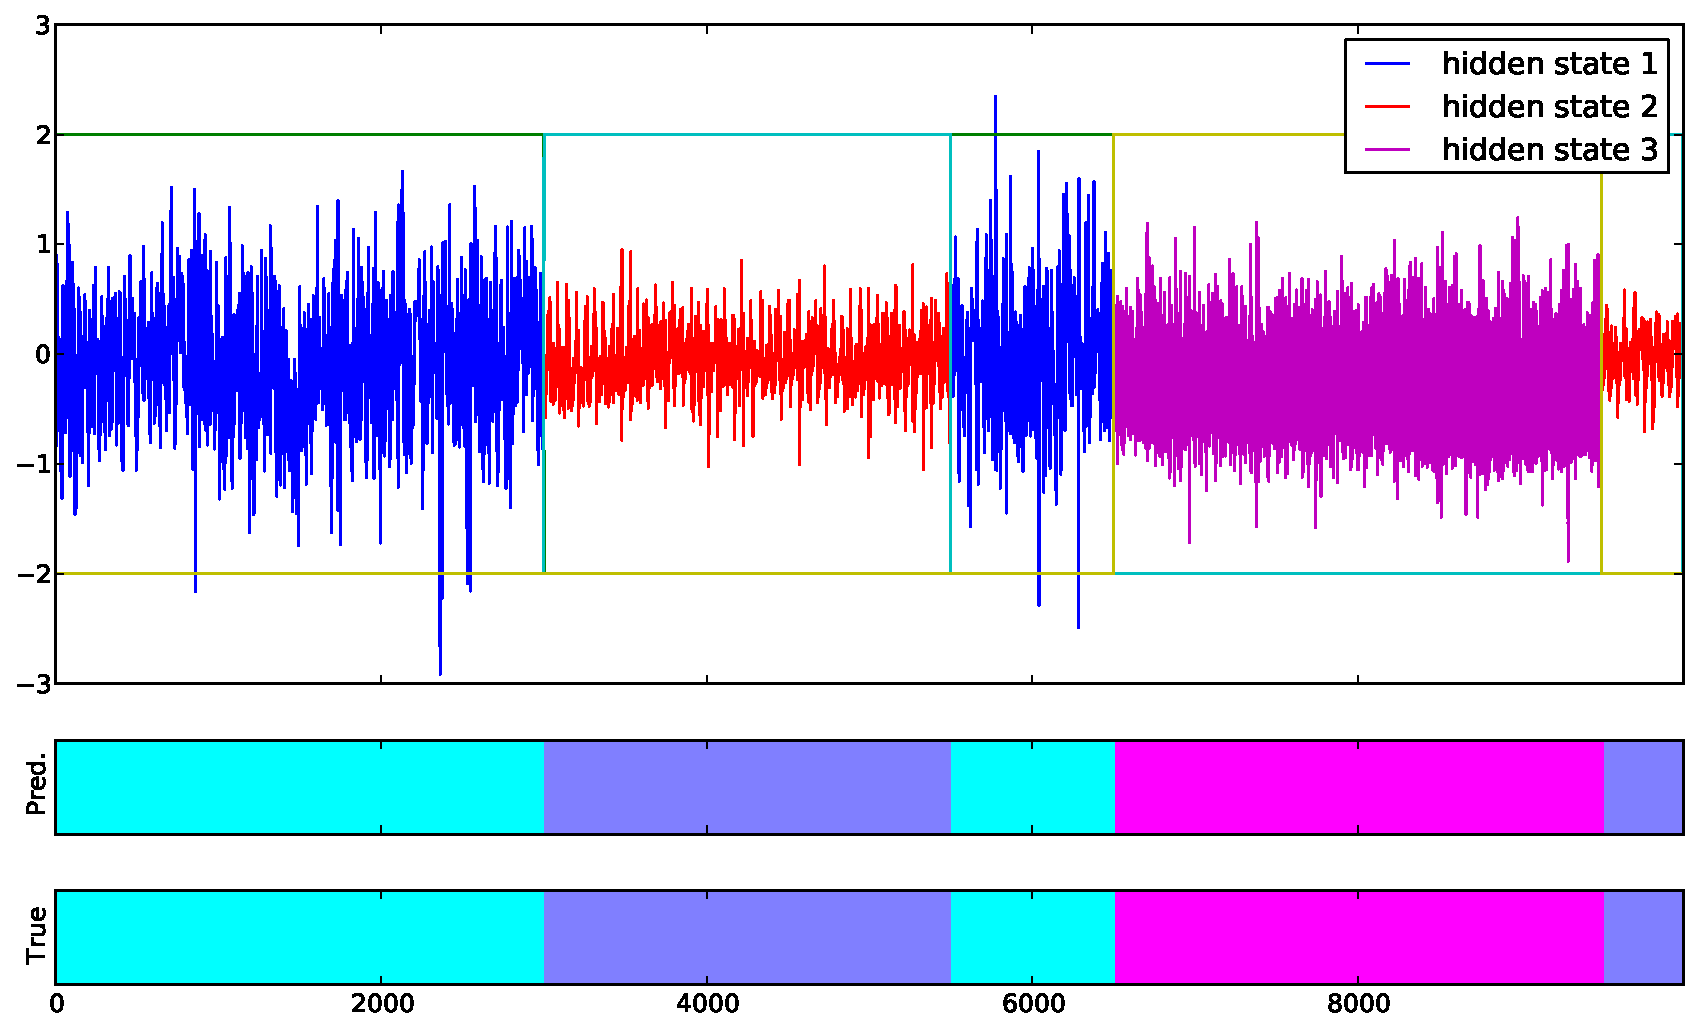
\includegraphics[width=0.8\linewidth]{images/MAP_PARAM_FREE_results_hard_activity_long_1,97_3_states.pdf}
    \label{fig:real-results-MAP}
\end{figure}

In contrast, an unregularized HMM performs poorly on the same task, since simply seeking to maximize the log-likelihood of the observations may require that states often transition between neighboring points. The segmentation errors can be seen at the bottom of Figure~\ref{fig:real-results-HMM}.

\begin{figure}[htbp]
  \caption{Segmentation of human activities accelerometer data using a standard HMM.}
  \centering
    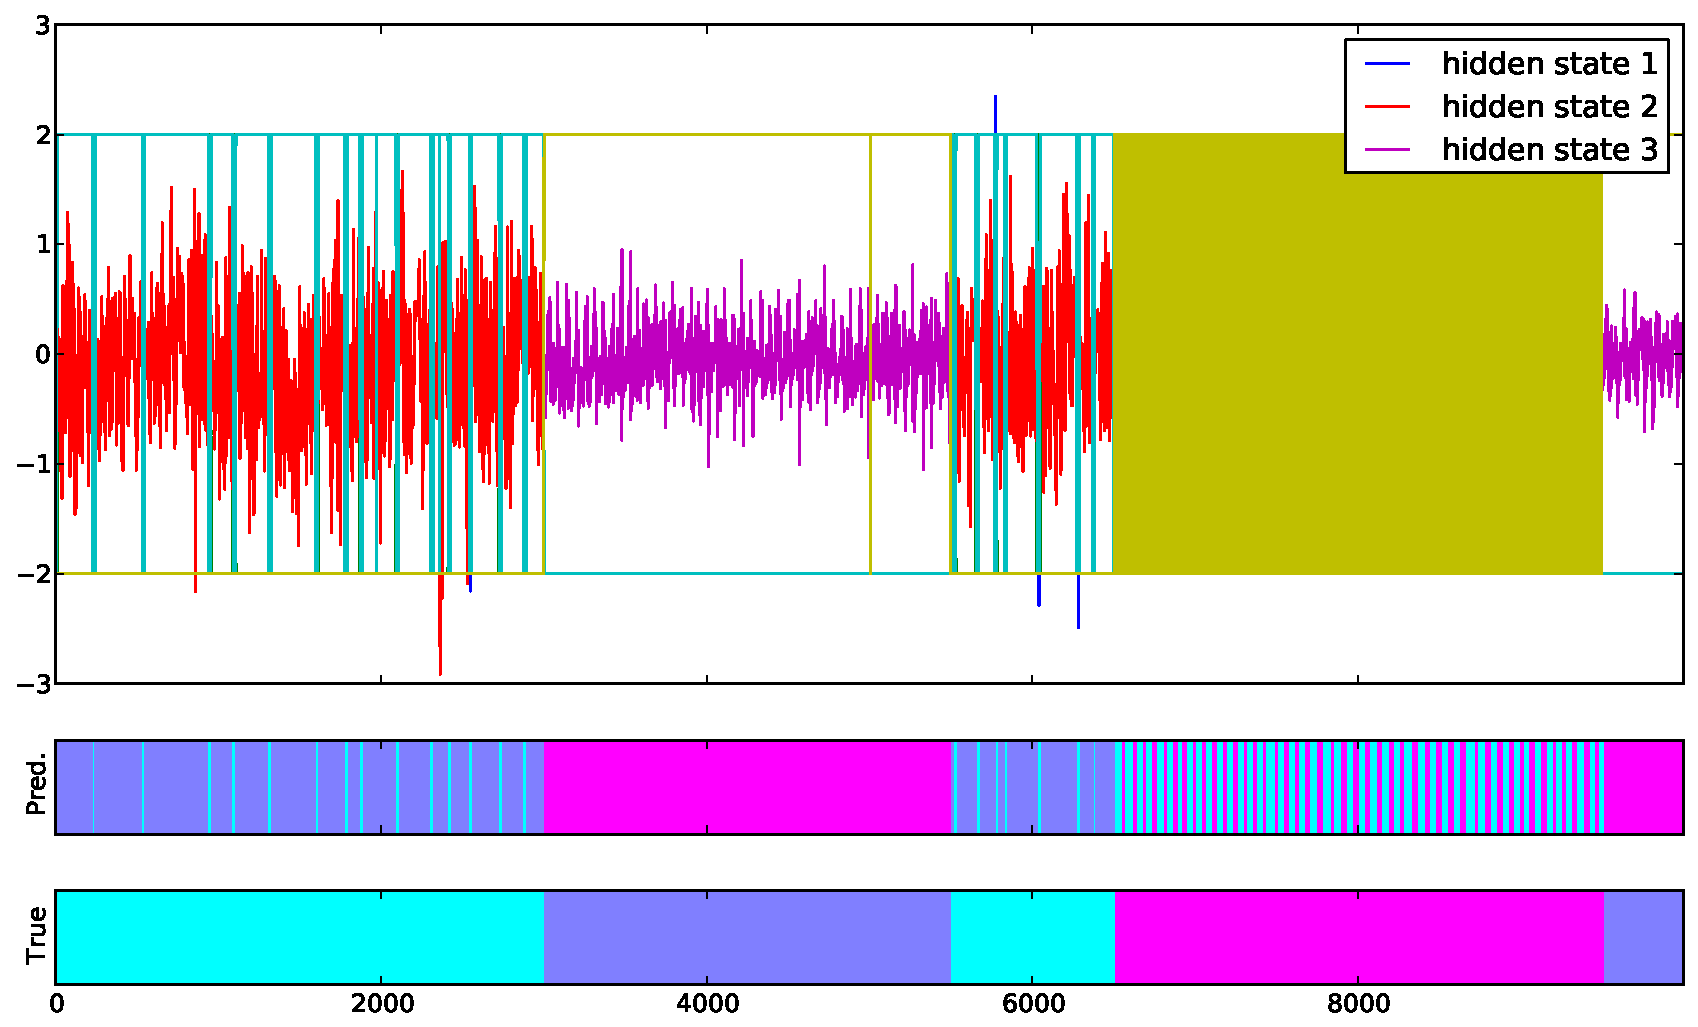
\includegraphics[width=0.8\linewidth]{images/std_hmm_results_hard_activity_3_states.pdf}
    \label{fig:real-results-HMM}
\end{figure}

\begin{table}[htbp]
\caption{Results from quantitative evaluation on multivariate human accelerometer data.}
\begin{tabular}{|lrrrrrr|}
\hline
\textbf{Method}                 & \textbf{Accuracy} & \textbf{SNR}  & \textbf{ASNR} & \textbf{SND}  & \textbf{VOI}    & \textbf{Perfect Segmentations}  \\ \hline
Standard HMM                    & 0.87              & 121.93        & 121.93        & 438.37        & 0.29            & 20/100                          \\ \hline
MAP HMM ($\zeta = 73$)        & \textbf{0.97}     & \textbf{1.02} & \textbf{1.05} & \textbf{0.19} & \textbf{0.06}   & \textbf{77/100}                   \\ \hline
Inertial HMM ($\zeta = 73$)     & \textbf{0.98}     & \textbf{1.02} & \textbf{1.05} & \textbf{0.18} & \textbf{0.06}   & \textbf{77/100}                 \\ \hline
\multicolumn{7}{l}{\begin{tabular}[c]{@{}l@{}}
    \vspace{0.05em}\\
    \textbf{Accuracy} = Average Accuracy (value of 1.0 is best)\\ 
    \textbf{SNR} = Average Segment Number Ratio (value of 1.0 is best)\\ 
    \textbf{ASNR} = Average Absolute Segment Number Ratio (value of 1.0 is best)\\ 
    \textbf{SND} = Average Segment Number Difference (value of 0.0 is best)\\ 
    \textbf{VOI} = Average Normalized Variation of Information (value of 0.0 is best)\\ 
    \textbf{Perfect Segmentations} = Total number of perfect/correct segmentations \end{tabular}} 
\end{tabular}
\label{tab:results}
\end{table}

Using the one hundred time series human activities dataset described in Section~\ref{sec:datasets}, we performed a quantitative analysis comparing the performance of standard and regularized MAP HMMs on the unsupervised segmentation task. The results are shown in Table~\ref{tab:results}. The MAP HMM achieved large gains in performance over the standard HMM model, with average accuracy of 97\%. Furthermore, the number of segments was close to correct on average, with a value near one in both the absolute and simple ratio case. On average, the MAP HMM over-segmented by only 0.19 segments, and was able to reproduce a perfect segmentation for 77\% of the test cases. The average normalized variation of information was low, at $0.06$.

Results for the inertial regularized HMM with pseudo-observations were almost identical, with slight differences in accuracy and segment number difference (SND). This is unsurprising, given the highly similar mathematical form of their final update equations.

In comparison, a standard hidden Markov model without inertial regularization achieved accuracy of 87\%, but with average absolute segment number ratio of 121.93 and average normalized variation of information value of $0.29$. On average, the segmentations given by the standard HMM differed by $438.37$ segments, compared to the fewer than one segment difference between the MAP HMM and the ground truth sequences. The standard HMM was only able to produce perfect segmentations in 20\% of the test cases.

Thus, the inertial regularization produces drastic improvements for unsupervised segmentation of human accelerometer activity data.

As a comparison, we also evaluated the MAP HMM with a small parameter of $\zeta = 3$. As expected, we achieved results nearer to that of the standard HMM, with average accuracy of 0.88, average normalized variation of information value of 0.23, average segment number ratio of 67.7 and perfect segmentation of 42/100 sequences.

\section{Discussion}

Our results demonstrate the effectiveness of inertial regularization on HMMs for time series segmentation. Although derived in two independent ways, the MAP regularized and pseudo-observation inertial regularized HMM converge on a similar maximum likelihood update equation, and thus, have similar performance. Either version can be used for segmentation tasks, according to user preference. 

The human activity task highlighted an issue with using standard HMMs for segmentation of time series with infrequent state changes, namely, over-segmentation. Incorporating regularization for state transitions provides a simple solution to this problem. Since our methods rely on changing a single update equation for a standard HMM learning method, they can be easily incorporated into HMM learning libraries with minimal effort. This ease-of-implementation gives a strong advantage over existing persistent-state HMM methods, such as the recent sticky HMM framework developed by Fox \emph{et al.}~\cite{fox2011sticky}.

\section{Related Work}

Hidden Markov models for sequential data have enjoyed a long history, gaining popularity with the widely influential tutorial of Rabiner~\cite{rabiner1989tutorial}. Specific to the work presented here, the use of regularization for HMM parameters received a general treatment in~\cite{MAP1994}, for both transition and emission parameters. Our work details a more specific version of the regularization, useful for state persistence. Neukirchen and Rigoll~\cite{neukirchen1999controlling} studied the use of regularization in HMMs for reducing parameter overfitting of emission distributions due to insufficient training data, but without an emphasis on inertial transitioning between states. Similarly, Johnson~\cite{Johnson07whydoesnt} proposed using Dirichlet priors on multinomial hidden Markov models as a means of enforcing sparse emission distributions. In contrast, Fox \emph{et al.}\ \cite{fox2011sticky} develop a Bayesian ``sticky'' HMM to provide inertial state persistence. They present a powerful method capable of learning a hidden Markov model without specifying the number of states or regularization strength beforehand, using a hierarchical Dirichlet process and truncated Gibbs sampling. Although our method is less powerful, requiring the number of states to be specified in advance, their method requires a more complex approach to learning the model. In contrast, our regularization only requires a small change to a single update equation, allowing drop-in regularization for standard Baum-Welch learning algorithms. 

\bibliographystyle{amsplain}
\bibliography{references}

\end{document}
